% !Mode:: "TeX:UTF-8"

%要运行该模板,LaTex需要安装CJK库以支持汉字.
%字体大小为12像素,文档类型为article
%如果你要写论文,就用report代替article
%所有LaTex文档开头必须使用这句话
\documentclass[12pt,twocolumn]{article}

%使用支持汉字的CJK包
\usepackage{CJKutf8}
\usepackage{indentfirst}
\usepackage[top=0.5in, bottom=0.5in, left=0.4in, right=0.4in]{geometry}
\usepackage[square,comma,numbers,sort&compress]{natbib}
\usepackage{graphicx}
\usepackage{booktabs}
\usepackage{tabularx}
\usepackage{enumitem}
\usepackage{titling}
\usepackage{subfigure}
\usepackage{ccaption}

\setlength{\parindent}{2em}
\setlength{\parskip}{0.5em}

\renewcommand{\contentsname}{目录}
\renewcommand{\listfigurename}{插图目录}
\renewcommand{\listtablename}{表格目录}
\renewcommand{\refname}{参考文献}
\renewcommand{\abstractname}{摘要}
\renewcommand{\indexname}{索引}
\renewcommand{\tablename}{表}
\renewcommand{\figurename}{图}

\setlength{\abovecaptionskip}{0em plus 0.3em minus 0.3em}
\setlength{\belowcaptionskip}{0em plus 0.3em minus 0.3em}
\setlength{\tabcolsep}{0.5em}
\setlength{\columnsep}{0.4in}

\linespread{1.1}

\setlist[1]{itemsep=0em,topsep=0em}

\renewcommand{\arraystretch}{1.3}

% make title left
\makeatletter
\renewcommand{\maketitle}{\bgroup\setlength{\parindent}{0pt}
\begin{flushleft}
  \LARGE {\textbf{\@title}}\vspace{1em}

  \normalsize{\@author}
\end{flushleft}\egroup
}
\makeatother

% change margin
\def\changemargin#1#2{\list{}{\rightmargin#2\leftmargin#1}\item[]}
\let\endchangemargin=\endlist

%开始CJK环境,只有在这句话之后,你才能使用汉字
%另外,如果在Linux下,请将文件的编码格式设置成GBK
%否则会显示乱码
\begin{CJK*}{UTF8}{gbsn}
\CJKindent
\CJKtilde

%这是文章的时间
%如果没有这行将显示当前时间
%如果不想显示时间则使用 \date{}
\date{}

%以上部分叫做"导言区",下面才开始写正文
\begin{document}

\twocolumn[
  \begin{@twocolumnfalse}
    %这是文章的标题
    \title{平行坐标综述}
    %这是文章的作者
    \author{赖楚凡\hspace{1em}袁晓如}
    %先插入标题
    \maketitle
    %\vspace{-4em}

    \begin{changemargin}{0.2in}{0in}
    {\bf 摘\hspace{1em}要:}
    \vspace{1em}

    {\bf 关键词:}
    \vspace{1em}
    \end{changemargin}

    %这是文章的标题
    \title{Parallel Coordinates}
    %这是文章的作者
    \author{Chufan Lai\hspace{1em}Xiaoru Yuan}
    %先插入标题
    \maketitle
    %\vspace{-4em}

    \begin{changemargin}{0.2in}{0in}
    {\bf Abstract: } 
    \vspace{1em}

    {\bf Keywords: }
    \vspace{2em}
    \end{changemargin}
  \end{@twocolumnfalse}
]

%再插入目录
%\tableofcontents
\section{引言}
\label{section:introduction}

在现实世界中,同一事物往往有多个不同的属性,要完整地描述该事物,需要记录其各个属性的信息。而这类具有多属性(维度)信息的数据,就称为多变量数据(Multivariate Data),或称高维数据(High-dimensional Data)。在传统的数据分析中,高维数据一般利用统计方法加以处理,并通过表格的方式呈现。但传统方法过于依赖自动算法,既无法结合用户的知识与判断,也不利于对抽象的高维信息的认知和理解。而信息可视化技术(Information Visualization)通过对高维数据的视觉呈现,辅以交互式的数据处理手段,能使用户充分参与到数据分析过程中,既加深了用户对数据的理解,也提高了分析的效率和可靠性。

高维数据一直是信息可视化领域的研究重点之一,其独有的两个特性:即维度数高、抽象性强,为可视化设计带来了巨大挑战。一方面,维度数的增长使得数据的信息量急剧增大,有限的显示空间只能表达一部分数据特征,而自动算法也会因为所谓的“维数灾难”(过高的复杂度、过低的采样率等~\citep{Bellman1962})而难以应用。另一方面,由于人无法感知高于三维的拓扑空间,高维的数据特征(如聚类、流型等)往往抽象而难以理解。针对这些挑战,领域内提出了各类高维可视化方法\citep{grinstein2001high},包括降维投影\citep{fodor2002survey}、散点图矩阵\citep{cleveland1988dynamic}、雷达图\citep{hoffman1999dimensional}、星型坐标\citep{kandogan2000star}等等。而由Inselberg等人提出的平行坐标~\citep{inselberg1985plane}(如图\ref{fig:PC_demo})也因其简单直观、可拓展性强等优点而被广泛应用于高维数据的可视分析中。

\begin{figure}[htb!]
\centering
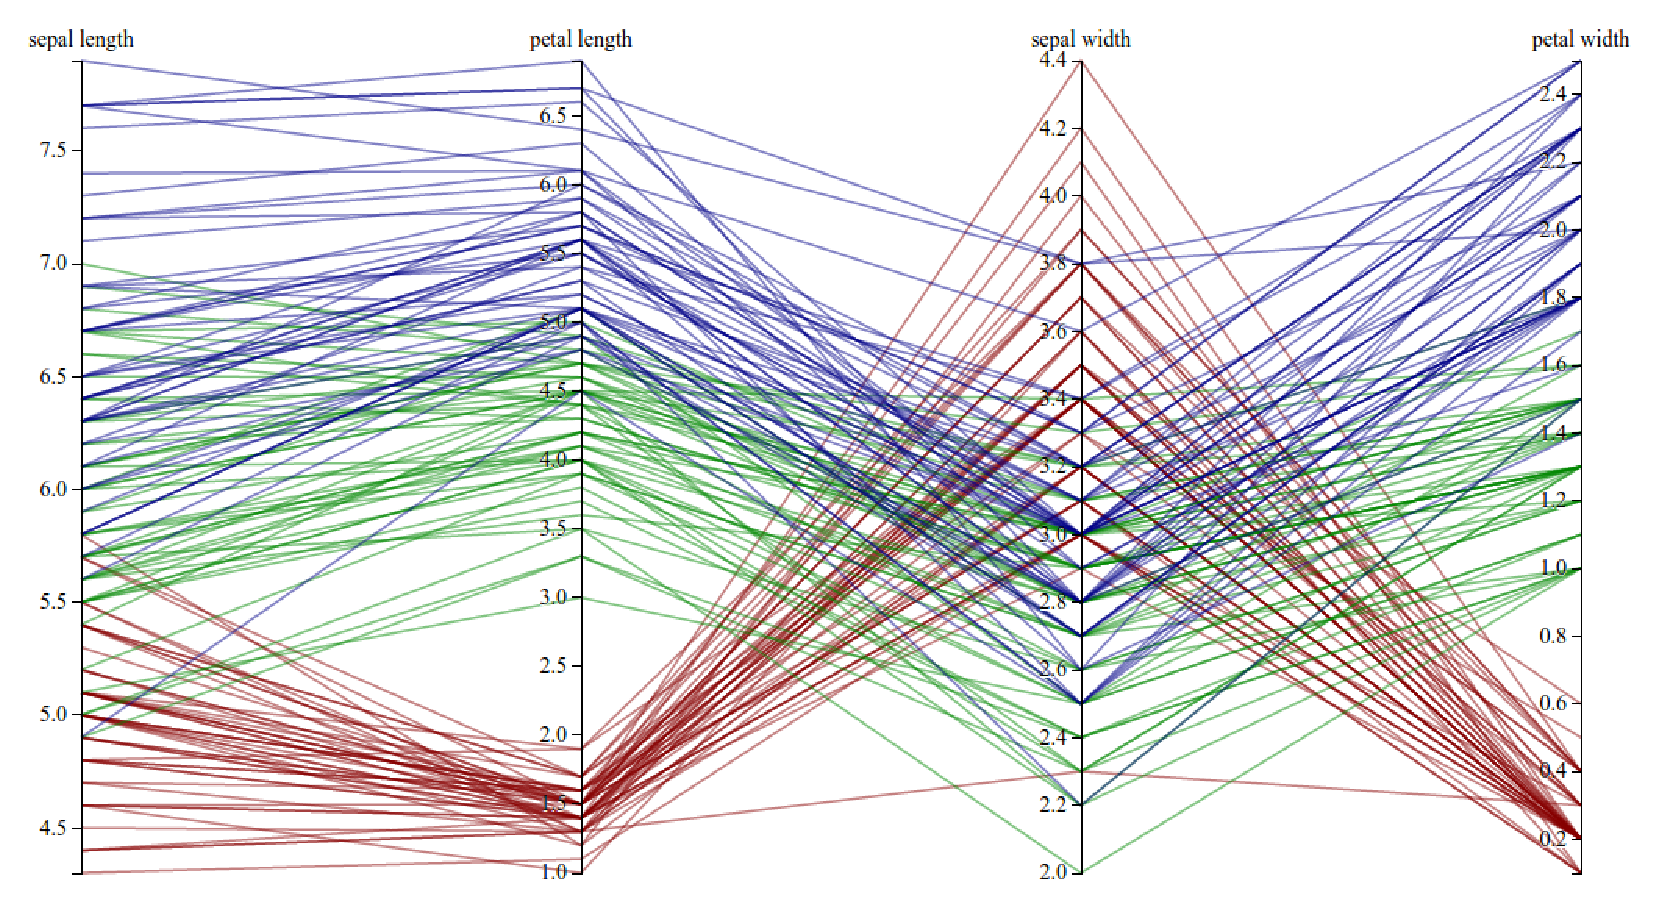
\includegraphics[width=0.9\linewidth]{images/PC_demo.eps}
\caption{\label{fig:PC_demo}平行坐标示例
}
\end{figure}

然而,相比于其他高维可视化形式,平行坐标的设计也存在种种缺点,譬如展现的信息量较少、容易出现视觉混杂(Visual Clutter)、数据特征不直观等等(详见第\ref{section:impro}节)。针对这些问题,领域内的学者们做了大量的研究工作,并提出了各种方法对平行坐标进行改进和延展。

本文基于一些已有的综述论文~\citep{grinstein2001high}~\citep{heinrich2013state}~\citep{siirtola2006interacting}~\citep{wong199430},并结合近年来的最新进展,将对平行坐标方面的研究工作进行比较、总结和展望。在文章的余下部分里:第\ref{section:basics&prob}节介绍了平行坐标的基本原理,并阐述其设计上存在的主要问题;第\ref{section:impro}节就平行坐标的不同部分,回顾了领域学者们为解决前述问题所作出的研究努力;第\ref{section:applications}节则介绍了平行坐标在不同领域内的应用现状;第\ref{section:challenges}节基于已有的研究和应用,探讨了仍然存在的挑战,以展望未来的研究动向和应用前景;最后,第\ref{section:conclusion}节对全文内容进行总结。

\section{基本原理及主要问题}
\label{section:basics&prob}
在这一节里,我们将从四个方面简要介绍平行坐标的设计。在此过程中,我们会逐步阐述平行坐标的几个主要问题。作进一步的探讨前,这里先简要介绍Jarke提出的的可视分析模型~\citep{van2005value}(如图\ref{fig:Vis_model})。在一个可视分析流程中,数据(Data)驱动了可视化展示(Visualization),用户对视图进行感知(Perception)并从中获取知识(Knowledge)。基于已有知识,用户可以通过交互探索(Exploration)来改变视图的参数设置(Specification),以产生新的可视化来发掘更多知识。由此可见,可视分析流程主要由四部分组成,分别是数据、视图、视觉感知和交互。本节余下内容以及第\ref{section:impro}节的内容都将按这四个部分展开。

\begin{figure}[!htb]
\centering
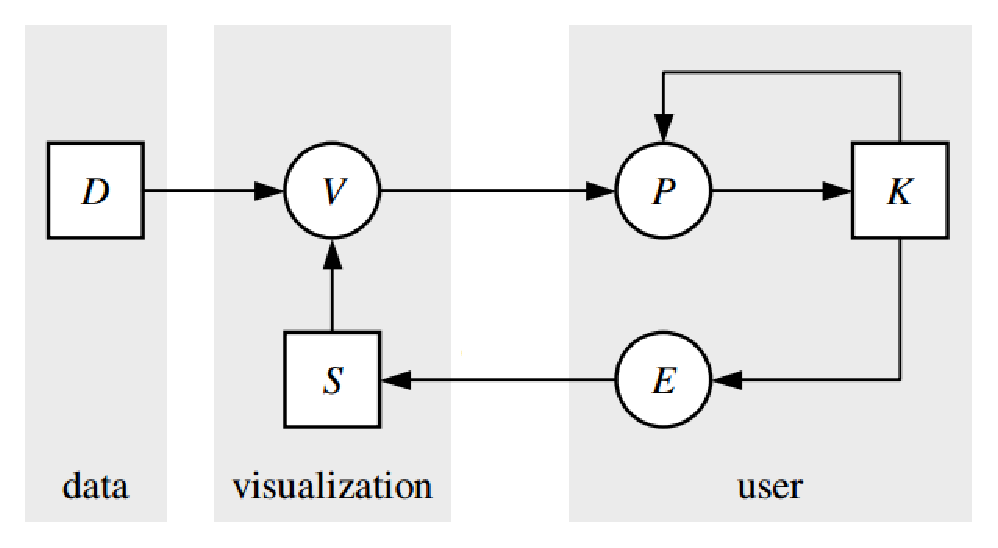
\includegraphics[width=0.9\linewidth]{images/Vis_model.eps}
\caption{\label{fig:Vis_model}可视分析模型。本图修改自Jarke~等人的论文~\citep{van2005value}~。
}
\end{figure}

\subsection{数据}
\label{subsection:dataBasics}
假设一个数据集有$m$个样本,每个样本有$n$个维度,则它可以记成一个$m \times n$的矩阵,其中每一行是一个样本,每一列代表一个维度。这样的矩阵又称为数据矩阵(data matrix),是平行坐标所处理的典型高维数据。数据的维度大致分为两种,即数值型维度~(Continuous Dimension,具有无数种取值,如身高、体重)和类别型维度~(Categorical Dimension,只有有限的取值,如国籍)。而一般的坐标轴只适用于数值型维度,类别型数据需要转换成数值型来表示,但往往会造成一定的误导(详见~\ref{subsection:designBasics}节),这使得平行坐标不适合表现类别型数据。其次,高维数据的产生往往伴随着其他类型的信息,譬如高维时空数据、高维网络数据、高维流场数据等等。如何拓展平行坐标以表现这些混合高维数据,也是研究的重点之一。除了不同的数据类型,数据的隐私性、不确定性,对大数据的处理等等,都是在数据方面的研究会涉及的课题。                                                                                                                                                                                                                                                                                                                                                                                                                                                                                                                                                                                                                                                                                                                                                                                                                                                                                                                                                                                                                                                                                                                                                                                                                                                                                                                                                                                                                                                                                                                                                                                                                                                                                                                                                                                                                                                                                                                                                                                                                                                                                                                                                                                                                                                                                                                                                                                                                                                                                                                                                                                                                                                                                                                                                                                                                                                                                                                                                                                                                                                                                                                                                                                                                                                                                                                                                                                                                                                                                                                                                                                                                                                                                                                                                                                                                                                                                               

\subsection{视图}
\label{subsection:designBasics}
正如第\ref{section:introduction}节所提到,人无法感知高于三维的拓扑关系。而传统的笛卡尔坐标系限定了各坐标轴必须相互垂直,这使得高维的坐标空间极为抽象和难以理解。平行坐标解决这一难题的方法,顾名思义,就是将各个维度的坐标轴平行放置,如图\ref{fig:PC_principle}所示。一个高维数据在各个坐标轴上均有取值,连接各取值点所形成的一条折线,即表达了这个数据。事实上,基于线和点的转化关系,平行坐标和笛卡尔坐标之间有很好的几何对称性,有兴趣的读者可参阅相关文献~\citep{inselberg1985plane}~\citep{inselberg2009parallel}。

\begin{figure}[!htb]
\centering
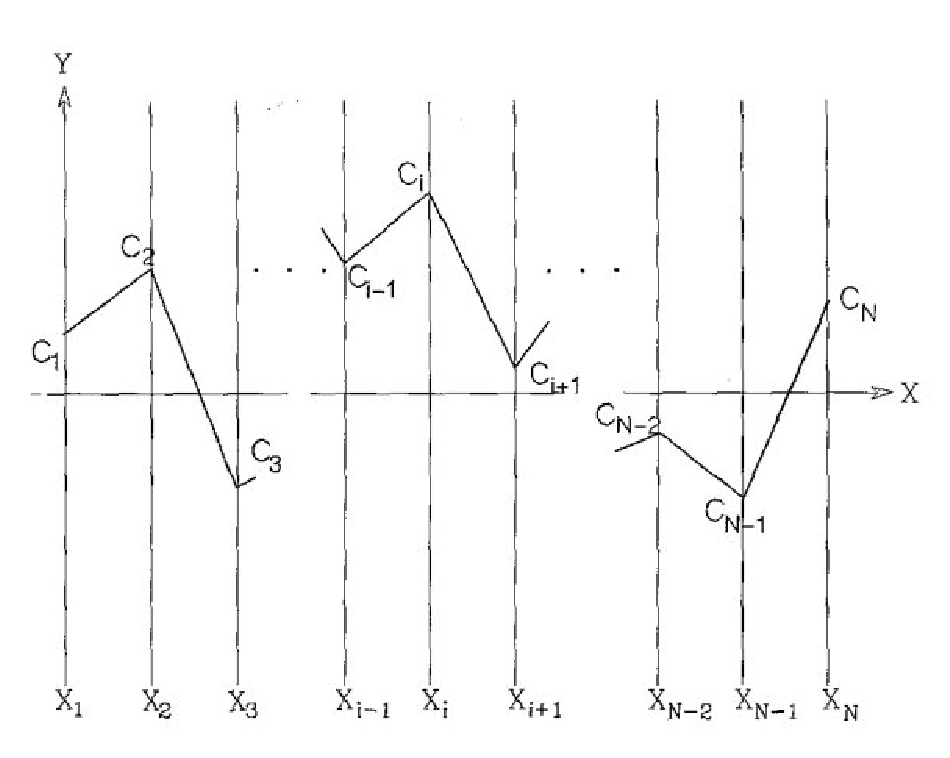
\includegraphics[width=0.9\linewidth]{images/PC_principle.eps}
\caption{\label{fig:PC_principle}平行坐标的构造原理。本图来源于Inselberg~等人的论文~\citep{inselberg1985plane}~。
}
\end{figure}

和其他高维可视化方法相比,平行坐标有几个突出的优点。首先,由于坐标轴的数量只受限于屏幕的横向分辨率,它相比于散点图矩阵等可以容易容纳更多维度,具有很强的可扩展性。其次,它完整地表达了数据在每个维度上的取值,相比于降维投影、雷达图等具有较低的不确定性和信息损失。最后,平行坐标构造简单、无需自动算法辅助,既方便使用也容易理解。

但相对地,平行坐标也存在一些明显的局限和缺点:

其一,当一个维度上有多个相同的取值时,多条折线汇合到一个点,直接观察将无法区分不同的数据走向。而在类别型的数据中,类似问题出现于每一个轴,导致大量线段完全重叠,用户甚至无法辨别其中的数据量(见图\ref{fig:PC_coincide})。这正是平行坐标不适合表现类别型数据的原因。

\begin{figure}[!htb]
\centering
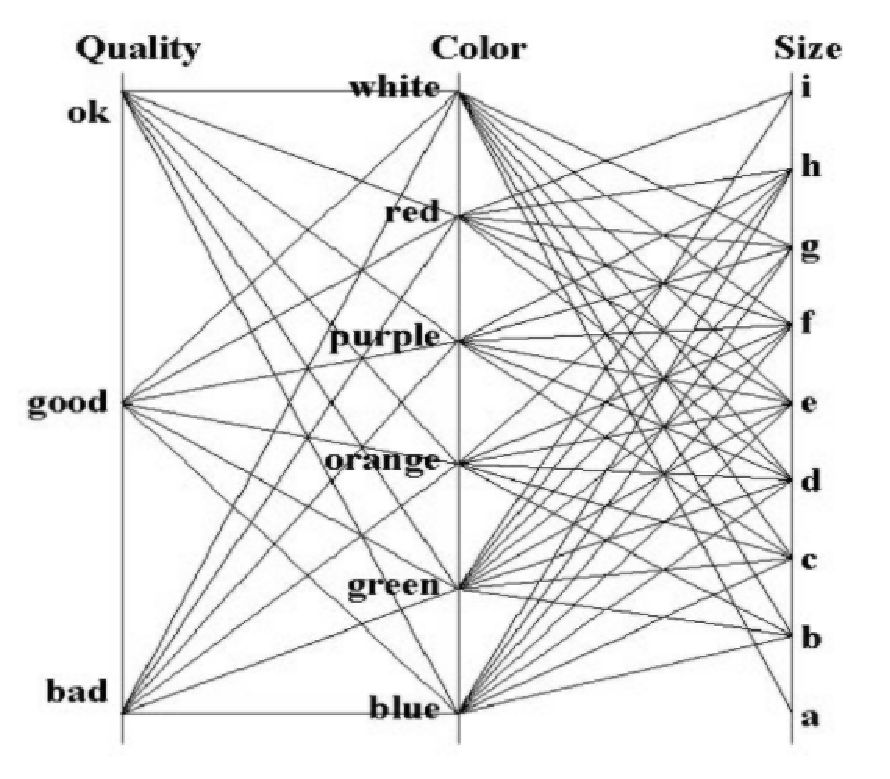
\includegraphics[width=0.6\linewidth]{images/PC_coincide.eps}
\caption{\label{fig:PC_coincide}类别型数据中的线段重合问题。本图来源于Rosario~等人的论文~\citep{rosario2004mapping}~。
}
\end{figure}

其二,每个数据用一条折线来表示,这会比散点形式占用更多的显示空间。当数据量增大时,视图很容易发生图元堆叠、导致视觉混杂(如图~\ref{fig:PC_clutter}),用户将无法从中得到有用的信息。由此可见,平行坐标对数据规模的扩展性较差。

\begin{figure}[!htb]
\centering
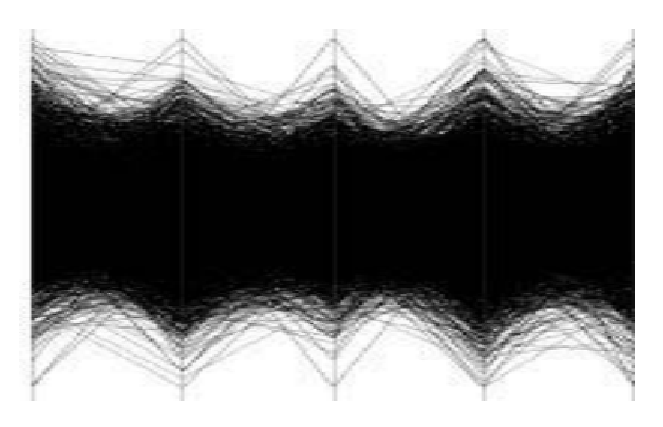
\includegraphics[width=0.8\linewidth]{images/PC_clutter.eps}
\caption{\label{fig:PC_clutter}视觉混杂问题。本图来源于Artero~等人的论文~\citep{artero2004uncovering}~。
}
\end{figure}

其三,平行坐标能够表现相邻维度间的关系,但信息量偏低。假设数据有$n$个维度,它们两两组合可得到$\frac{n(n-1)}{2}$个二维子空间,散点图矩阵能容纳其中的所有信息。但在平行坐标里,用户无法观察两个不相邻维度间的关系,因此只能看到$(n-1)$个二维子空间。换言之,平行坐标只表现了$\frac{2}{n}$的维度关系,不恰当的坐标轴排序很容易掩埋重要的相关性信息(如图\ref{fig:PC_reordering})。

\begin{figure}[!htb]
\centering
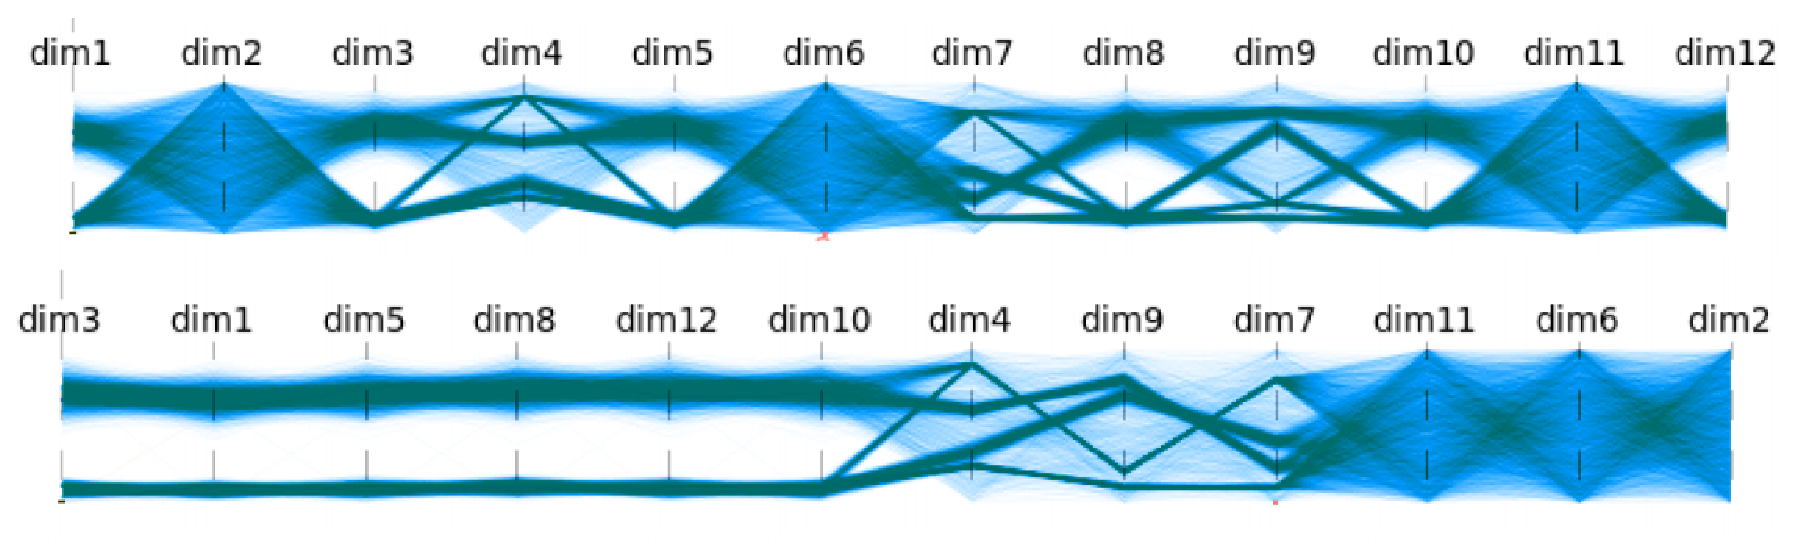
\includegraphics[width=1.0\linewidth]{images/PC_reordering.eps}
\caption{\label{fig:PC_reordering}不同坐标轴顺序对平行坐标的影响。其中上、下图分别为重排序前、后的视图,可见排序后各个维度的相关性和差异性更为明显。本图修改自Ferdosi~等人的论文~\citep{ferdosi2011visualizing}~。
}
\end{figure}

最后,除了排序上的变化,坐标轴的放置还存在许多可能性。平行坐标的出现启发了大量对非垂直坐标系、甚至是非直线坐标轴的的研究,这些都将在第~\ref{section:impro}节中加以讨论。

\subsection{感知}
\label{subsection:perceptionBasics}

针对平行坐标的感知研究主要有两种,一是视觉感知的有效性评估,二是数据特征的刻画和提取。

\begin{figure}[!htb]
\centering
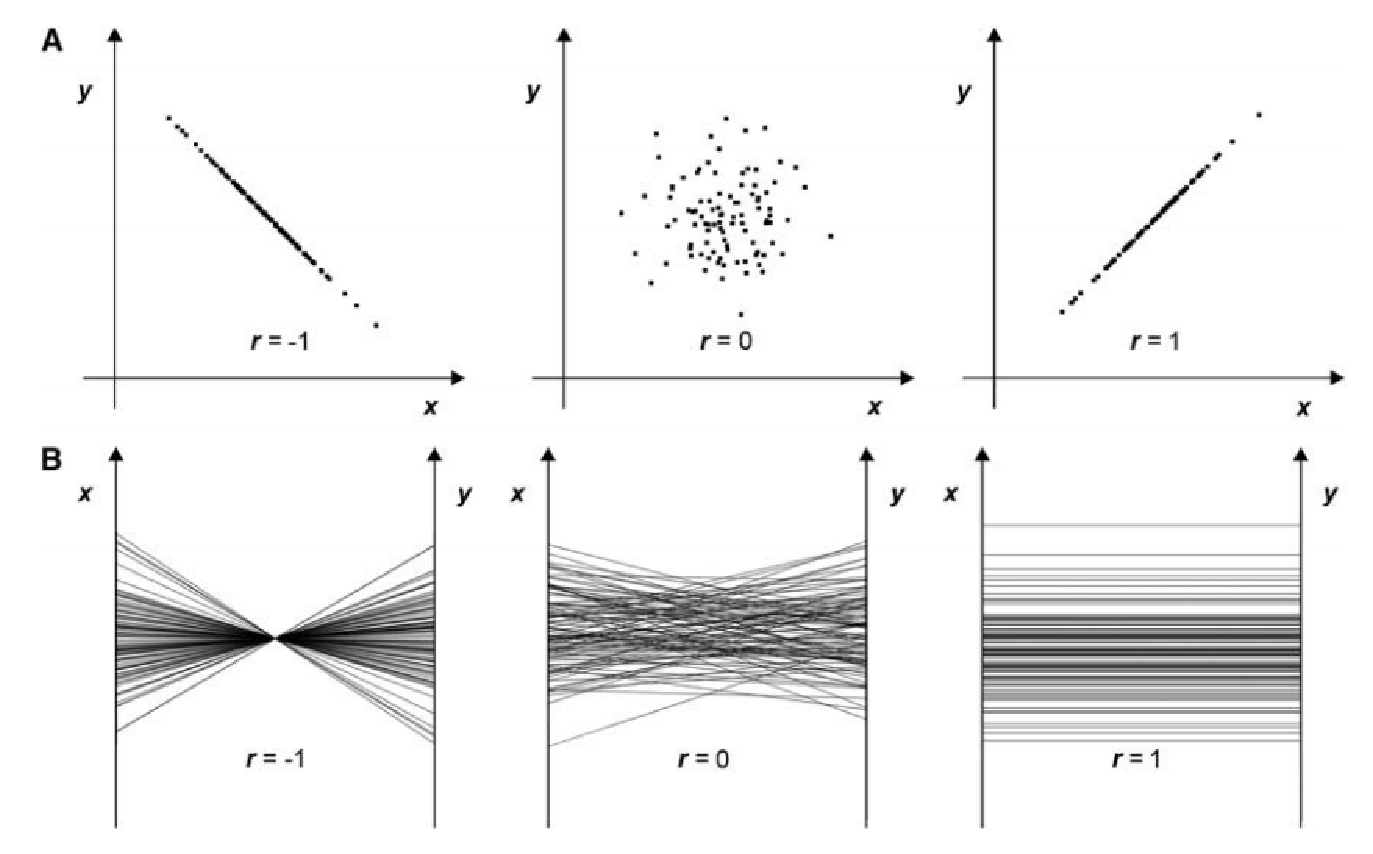
\includegraphics[width=1.0\linewidth]{images/PC_correlation.eps}
\caption{\label{fig:PC_correlation}维度相关性的解读。A、B两行分别显示了不同的相关关系下数据在散点图和平行坐标中的分布。本图来源于Li~等人的论文~\citep{li2010judging}~。
}
\end{figure}

在平行坐标里,能观察到的数据特征主要有两种,即聚类信息和相关关系。一方面,相似的折线形成线簇,代表着不同的聚类,反映了数据趋势、异常点等行为。但要观察到聚类,必须先处理好前面提到的视觉混杂问题,使隐含的聚类能被凸显出来。另一方面,相邻坐标轴之间的线段走向能反映这两个维度的相关关系(如图\ref{fig:PC_correlation})。但用户对相关性的感知是否准确,和其他方法相比是否更有效等等,都需要通过实验来评估。除此之外,还有很多有意义的数据特征无法通过简单的聚类或相关来描述。而已有的特征也需要相应的自动提取算法,来遍寻和评估不同的参数设置(如不同的维度排序),以找到特征明显、信息量大的视图。

\subsection{交互}
\label{subsection:interactionBasics}

基于已有的观察,用户通过交互来改变视图,以发掘更多信息。平行坐标提供两种基本的交互功能,即数据刷选和坐标轴排序。对于刷选,用户需要给每个坐标轴限定取值范围~\citep{martin1995high}。这相当于在高维空间中建立一个超立方体(Hypercube)包围盒,同时满足各维度条件的数据才会被选中。这样的方式虽然逻辑简单,但操作繁琐、缺乏灵活性,用户既无法选中任意形状的数据区域,也无法根据其他数据特征来选择数据。除了刷选,用户还可以手动调整坐标轴的顺序。但这在数据维度较高时并不现实,用户很难通过交互来发现合适的排序。

\section{平行坐标的相关研究}
\label{section:impro}

针对前一节中提出的各种问题,领域学者们做了许多研究工作来对平行坐标进行改进和延展。这一节将详细地回顾这些工作,并对它们进行比较和总结。为了保持行文结构、方便读者对照理解,这一节依然按数据、视图、感知和交互四个部分来展开。

\subsection{数据}
\label{subsection:dataImpro}

对数据的研究主要关注三个方面:不同的数据类型、不确定性与数据隐私、以及绘制效率。

\subsubsection{不同的数据类型}

正如~\ref{subsection:designBasics}节所述,由于折线重叠问题,平行坐标并不适合表现类别型数据。在这种数据里,大量样本具有相同的类别,它们相互之间无法被区分。但事实上,这些数据的分析重点并不在于单个样本,而是同一类样本的集合,因此需要在平行坐标里加入表达集合关系的元素。一方面,可以对类别型维度进行量化~\citep{rosario2004mapping},以表达不同类别之间的关系(如图\ref{fig:PC_Data_Quantification}),但用户依然无法判断每个类别内的数据量。

\begin{figure}[!htb]
\centering
\subfigure[]{
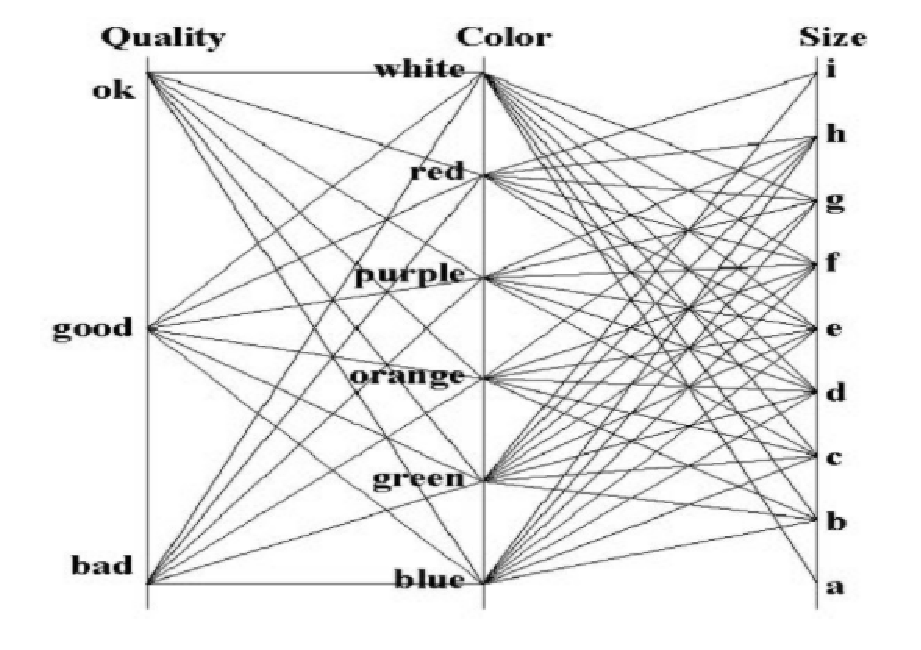
\includegraphics[width=0.47\linewidth]{images/PC_Data_Quantification1.eps}}
\subfigure[]{
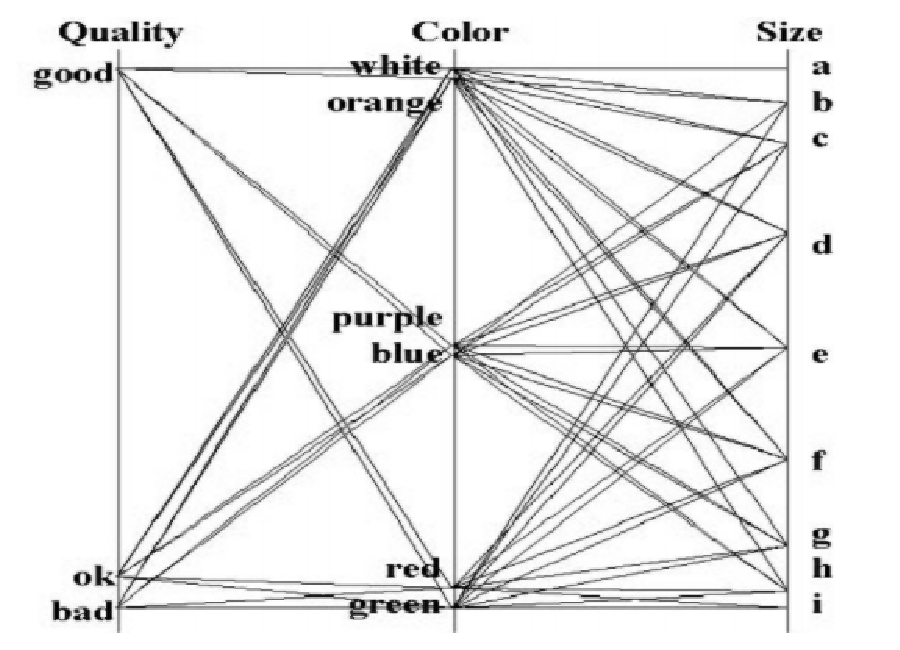
\includegraphics[width=0.47\linewidth]{images/PC_Data_Quantification2.eps}}
\caption{\label{fig:PC_Data_Quantification}类别型维度在量化前后的对比。本图源自Rosario等人的论文~\citep{rosario2004mapping}~。}
\end{figure}

\begin{figure}[!htb]
\centering
\subfigure[平行集合]
{\label{fig:PC_Data_ParallelSet}
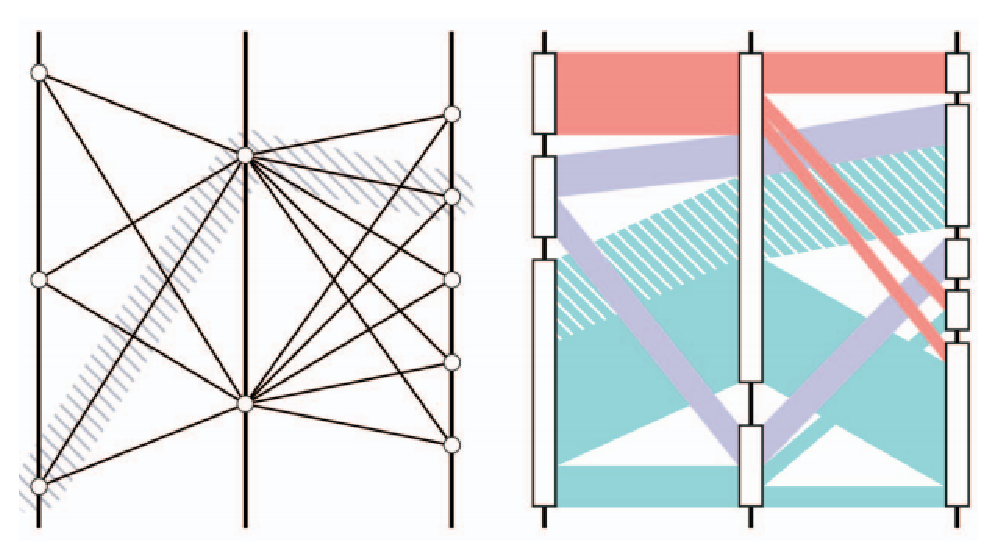
\includegraphics[width=0.9\linewidth]{images/PC_Data_ParallelSet.eps}}
\subfigure[统一角度图]
{\label{fig:PC_Data_CommonAnglePlot}
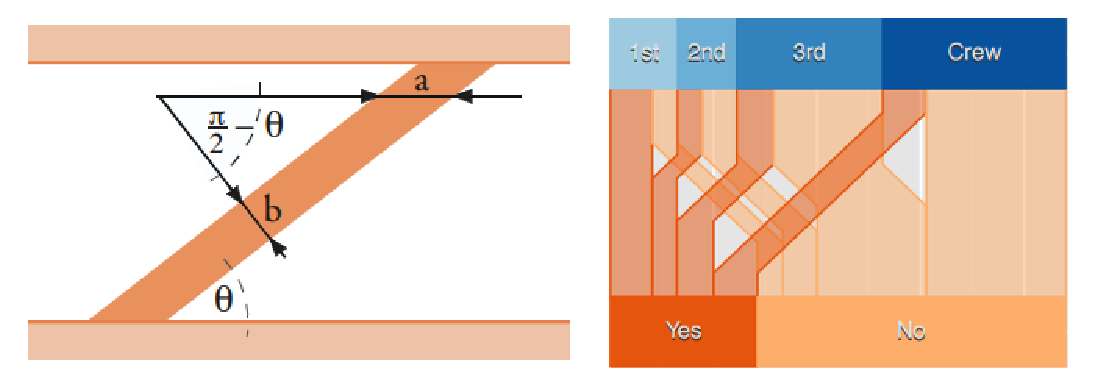
\includegraphics[width=0.9\linewidth]{images/PC_Data_CommonAnglePlot.eps}}
\caption{平行集合及其改进版本,用以在平行坐标框架下表现类别型数据。图(a)、(b)分别来自论文~\citep{kosara2006parallel}和~\citep{hofmann2013common}。}
\end{figure}

另一方面,样本数量可以用折线宽度来表示,即平行集合(Parallel Set)~\citep{kosara2006parallel}~\citep{bendix2005parallel}的形式,各个集合之间的交错、包含等逻辑关系也更为明显(如图\ref{fig:PC_Data_ParallelSet})。而Hofmann等人~\citep{hofmann2013common}指出,斜线段的宽度并不对应它所代表的数据量(比较图\ref{fig:PC_Data_CommonAnglePlot}中的$a$、$b$两段)。他们提出用统一的角度来绘制折线,即统一角度图(Common Angle Plot)的形式,使用户能通过直线部分的宽度来准确感知集合的大小。

除了类别型数据,时变数据也是一类重要的拓展,具体方法可分为静态和动态两种。其中静态的展示需要引入时间轴、并同时绘制所有时刻的数据,只是对时间轴的处理各有不同(见图\ref{fig:PC_Data_Time5})。

\begin{figure}[!htb]
\centering
\subfigure[]{
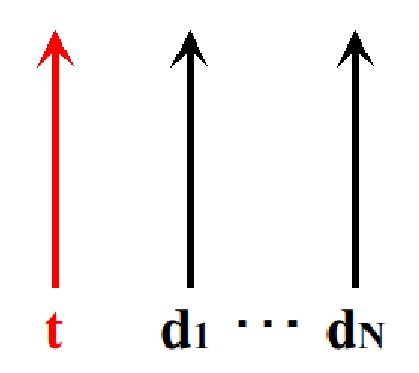
\includegraphics[width=0.25\linewidth]{images/PC_Data_Time5_1.eps}}
\subfigure[]{
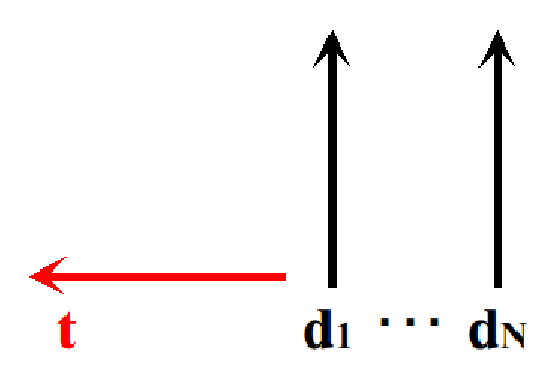
\includegraphics[width=0.35\linewidth]{images/PC_Data_Time5_2.eps}}
\subfigure[]{
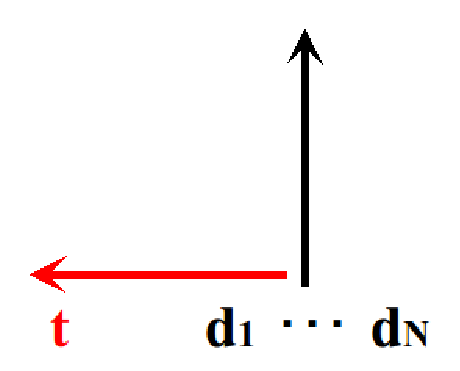
\includegraphics[width=0.28\linewidth]{images/PC_Data_Time5_3.eps}}
\caption{\label{fig:PC_Data_Time5}时变平行坐标的三种静态展示方式:(a).时间轴平行于属性轴;(b).时间轴在坐标平面内垂直于属性轴;(c).时间轴垂直于坐标平面。}
\end{figure}

最简单的方式莫过于将时间轴看作一个平行轴,但各个时刻的数据被同等对待,不利于凸显数据的变化信息。Johansson等人~\citep{johansson2007depth}提出利用不透明度和色调等来区分数据变动的时间范围(如图~\ref{fig:PC_Data_Time3})。用户可以直观地看出变化的频率和趋势,但不同时刻的数据依然会相互遮挡。

\begin{figure}[!htb]
\centering
\subfigure[]{
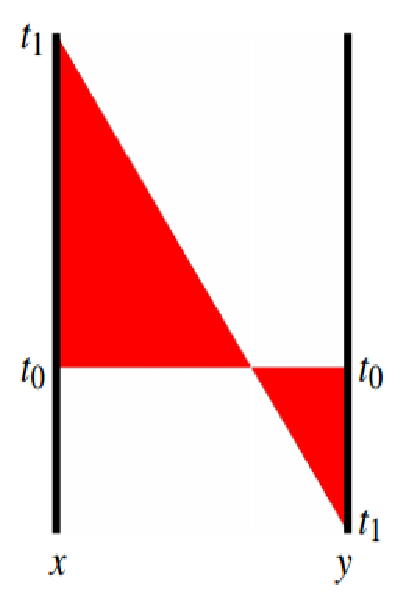
\includegraphics[width=0.3\linewidth]{images/PC_Data_Time4.eps}}
\subfigure[]{
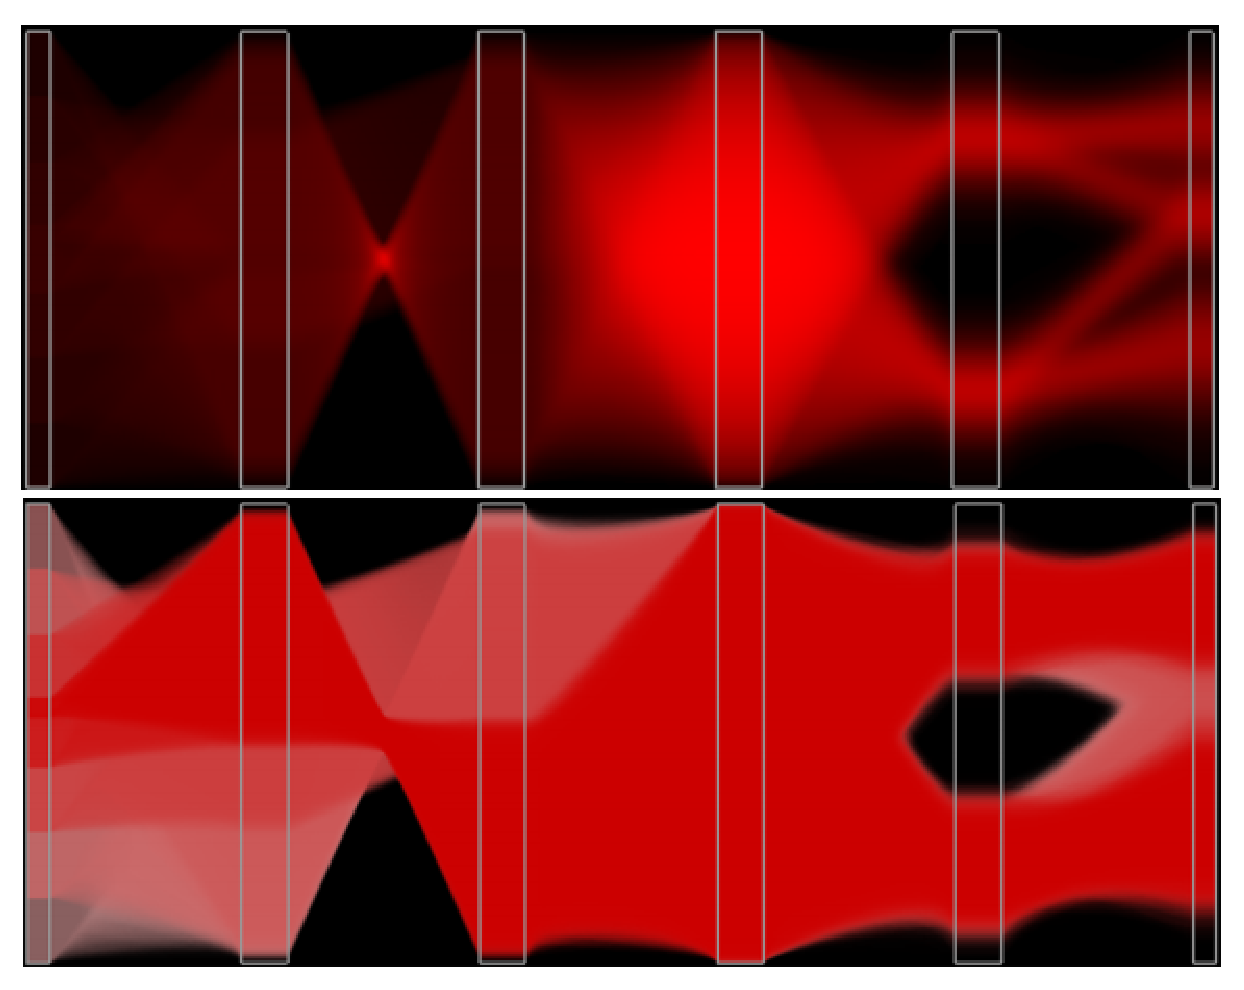
\includegraphics[width=0.6\linewidth]{images/PC_Data_Time3.eps}}
\caption{\label{fig:PC_Data_Time3}用不透明度和色调刻画数据变动。其中折线变化用多边形表示(如图(a)),不透明度刻画了变化的频率,不同的色调则代表不同的时刻(如图(b))。本图来源于Johansson~等人的论文~\citep{johansson2007depth}~。}
\end{figure}

为防止遮挡,也可以结合折线图(Line Chart),用多个轴表示一个维度的时变信息~\citep{edsall2003parallel}~\citep{dietzsch2009spray}(如图\ref{fig:PC_Data_Time1}),但同一维度的重复出现会大大降低视图的可扩展性。

\begin{figure}[!htb]
\centering
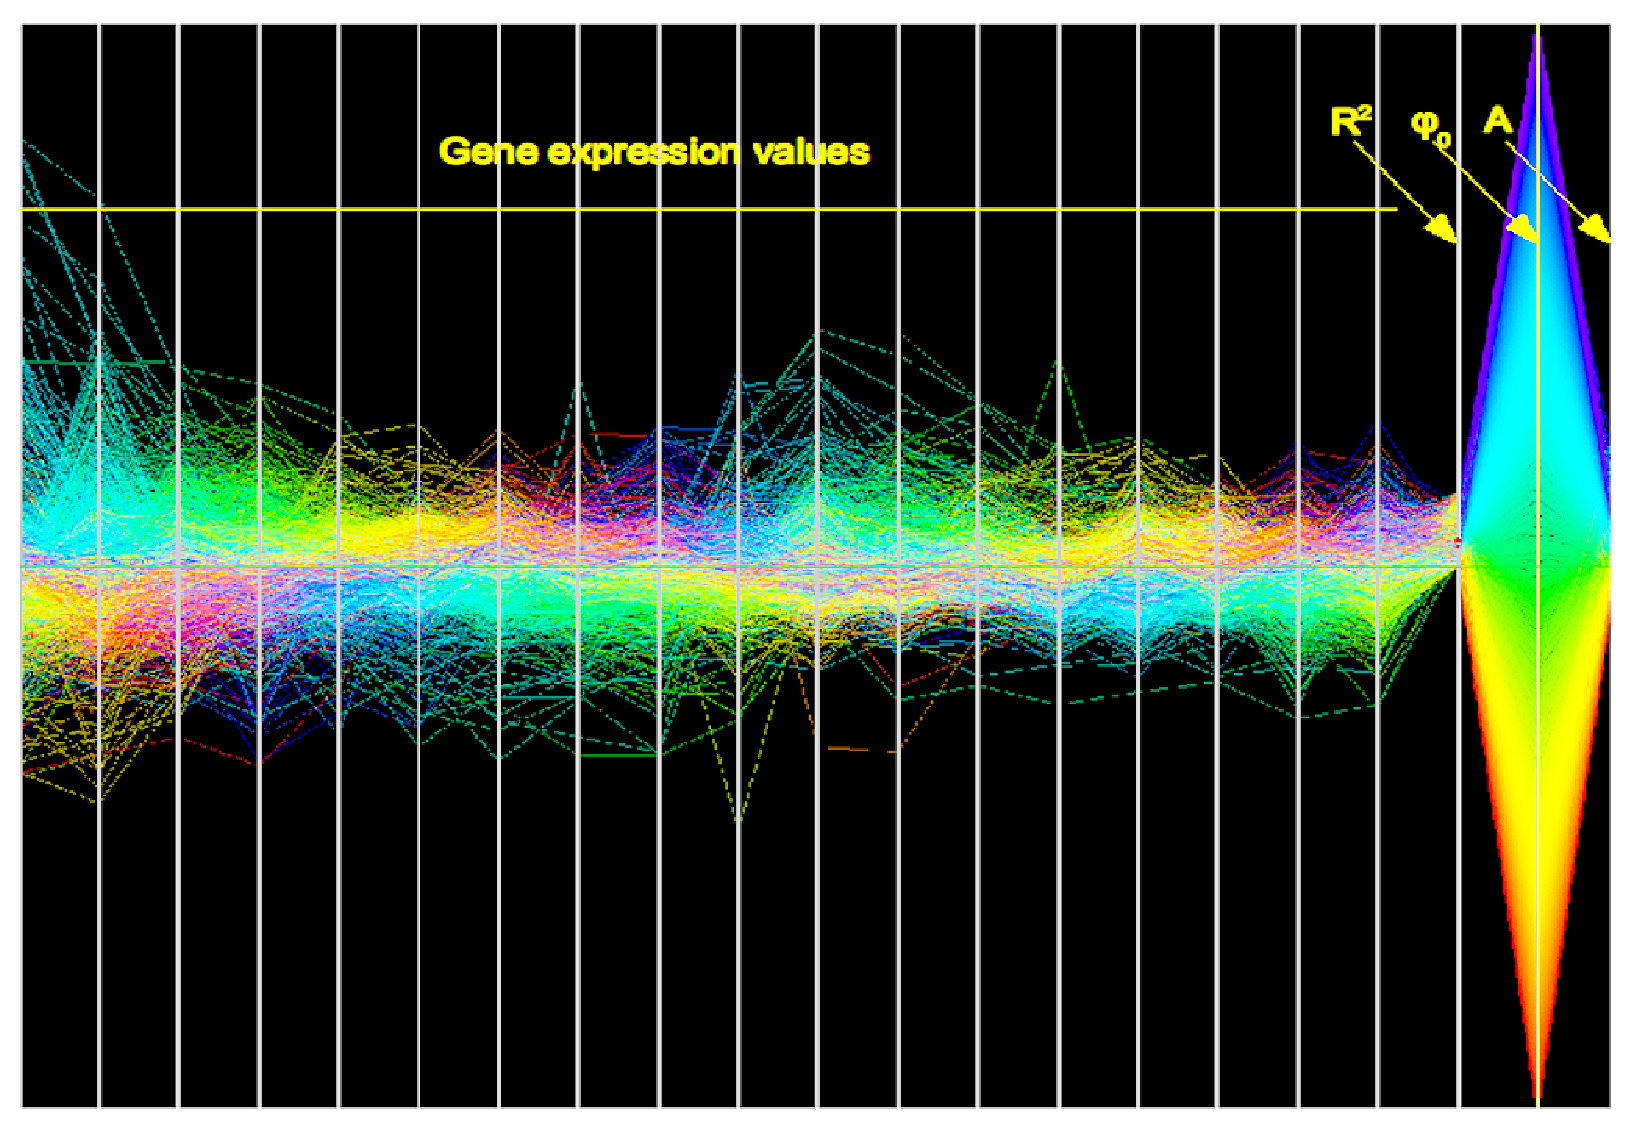
\includegraphics[width=0.9\linewidth]{images/PC_Data_Time1.eps}
\caption{\label{fig:PC_Data_Time1}在平行坐标中嵌入折线图。本图来源于Dietzsch~等人的论文~\citep{dietzsch2009spray}~。
}
\end{figure}

进一步地,Wegenkittl等人~\citep{wegenkittl1997visualizing}令时间轴垂直于坐标平面,提出了三维时变平行坐标的形式(如图~\ref{fig:PC_Data_Time2})。其中每条折线沿时间轴演化会形成一个曲面,该曲面即表达了时变高维的所有信息。但多个不同的曲面很容易交错重叠而难以观察,使其不适用于数据量大的情形。

\begin{figure}[!htb]
\centering
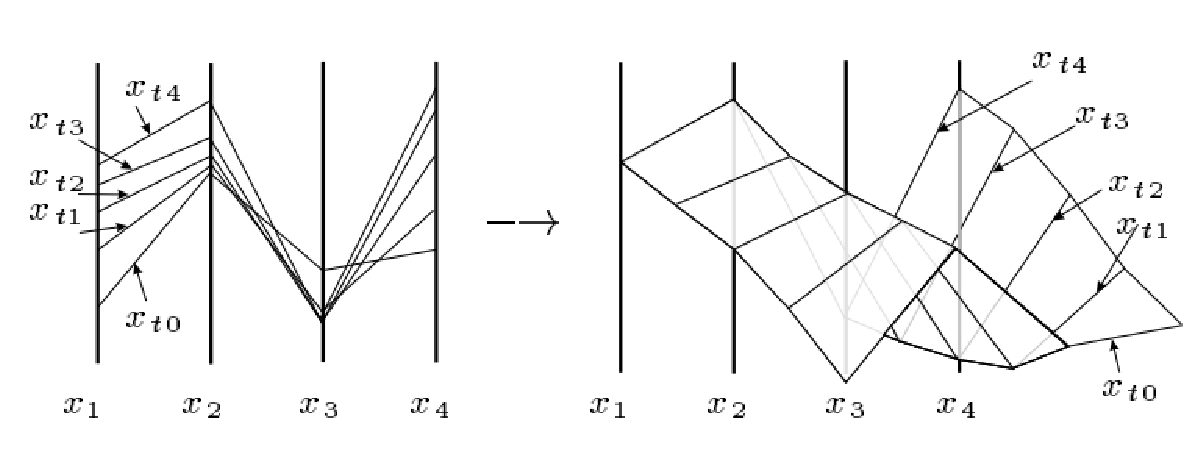
\includegraphics[width=1.0\linewidth]{images/PC_Data_Time2.eps}
\caption{\label{fig:PC_Data_Time2}三维时变平行坐标。图中$x_1$至$x_4$表示不同维度,$t_1$至$t_4$为不同的时刻。本图来源于Wegenkittl~等人的论文~\citep{wegenkittl1997visualizing}~。
}
\end{figure}

除了静态展示,还可以用动画来表现数据变化~\citep{barlow2004animator}。但视觉的瞬变使用户难以同时跟踪多个维度的变动,在维数较高、变动剧烈的情况下尤为如此。为每个维度提供额外的时变直方图~\citep{blaas2008extensions}可以缓解这一问题,但这又割裂了时变信息与维度关系。总的来说,以上方法都各有优劣,但还没有一个较为全面的方式来展现时变平行坐标。

还有一类拓展在于连续型数据。在科学数据(Scientific Data)里,所有样本可能都来自同一个数据域(Data Domain,如流场、物体表面等)。平行坐标能够逐个描绘这些样本,但无法展现通过插值重构出来的连续数据域,即所谓的“连续型数据”(Continuous Data)。绘制连续型数据的概念最早由Bachthaler等人~\citep{bachthaler2008continuous}提出并应用在散点图中。他们基于离散的样本,建模估计、并以颜色表现了视图各处的密度。基于这一研究,Heinrich等人利用散点图和平行坐标的几何对称性,发展出连续型平行坐标~\citep{heinrich2009continuous}的形式(如图\ref{fig:PC_Data_Continuous2})。后来的研究~\citep{lehmann2011features}则进一步揭示了这两种连续视图之间的密切联系。

\begin{figure}[!htb]
\centering
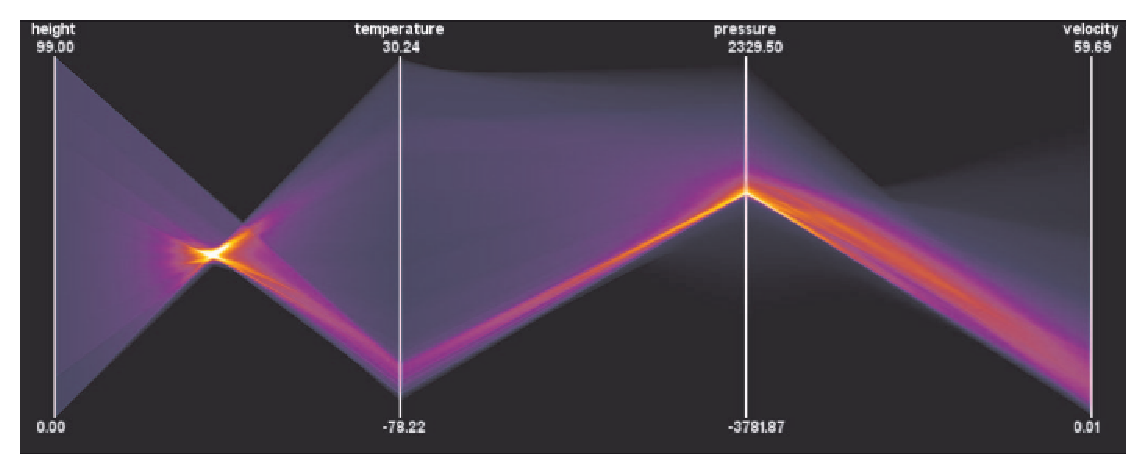
\includegraphics[width=1.0\linewidth]{images/PC_Data_Continuous2.eps}
\caption{\label{fig:PC_Data_Continuous2}连续型平行坐标。本图来源于Heinrich~等人的论文~\citep{heinrich2009continuous}~。
}
\end{figure}

相比于传统形式,连续型平行坐标可以在样本较少的情况下重构出精度较高的原数据域,而且能避免视图混杂问题(见~\ref{subsection:dataImpro}节),也具有较好的可扩展性和渲染效率。但它无法给出单个样本的信息,也不支持传统的交互和分析方法(如刷选、聚类等),在可用性上有一定的局限。

\subsubsection{不确定性与数据隐私}

无论什么类型的数据,都会在其采集和处理的过程中,因为种种原因(测量误差、样本随机性等)产生不同程度的不确定性。从结果推测的原数据因而会呈现概率分布,而这些分布则需要通过样本重构来得到。前面关于连续型数据的研究~\citep{bachthaler2008continuous}~\citep{heinrich2009continuous}都假定数据域是被充分均匀采样的,并采取线性插值的方法来进行重构。但这些假定都基于格点型的数据(Grid Data),对于不充分、非均匀采样的情形并不适用。

\begin{figure}[!htb]
\centering
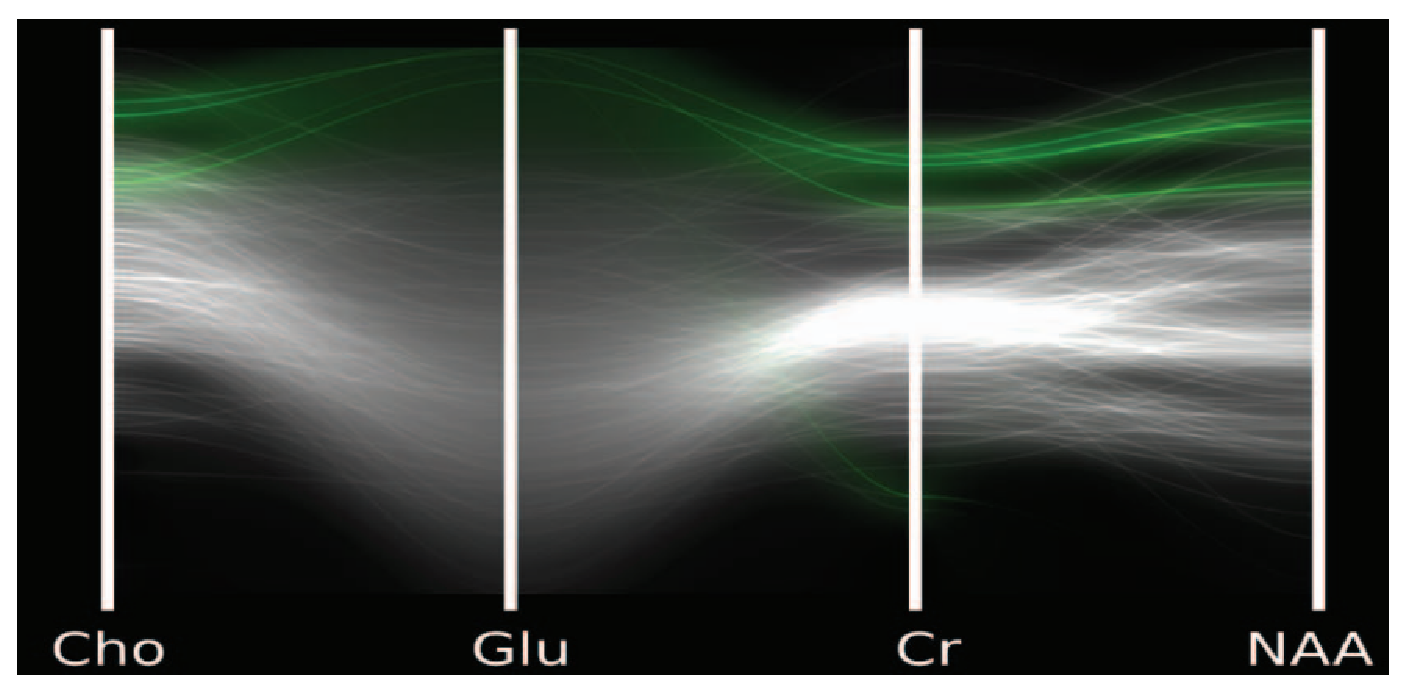
\includegraphics[width=1.0\linewidth]{images/PC_Data_Uncertainty.eps}
\caption{\label{fig:PC_Data_Uncertainty}平行坐标表现数据不确定性。本图来源于Feng等人的论文~\citep{feng2010matching}~。
}
\end{figure}

对于一般的数据,Feng~\citep{feng2010matching}等人提出用高斯核密度估计(Kernel Density Estimation)来进行重构,并利用连续型平行坐标的技术来绘制数据分布(如图\ref{fig:PC_Data_Uncertainty})。视图中密度越高的区域,其数据分布越集中,不确定性也越低。除此之外,他们还对这一技术作了曲线形式的拓展,并加入了基于密度的刷选、高亮等交互方式。

不确定性往往是分析人员极力避免的因素。但反过来,我们也可以制造“额外的”不确定性,通过隐藏样本数据来保护其中的隐私信息。上述基于密度的方法给出了原数据域的分布,其信息量甚至大于样本数据,因此不适合隐私保护。Dasgupta等人~\citep{dasgupta2011adaptive}提出通过聚类来封装底层数据(如图~\ref{fig:PC_Data_Privacy}),并重新设计了相应的交互手段,以抵御不同形式的隐私攻击。但他们设置的信息保护机制过于复杂,导致视图难以理解,大大降低了其可用性。相比于隐藏单个数据,另一种方案在于只显示部分样本,或是对重构的数据域进行再采样~\citep{heinrich2011progressive}来获得虚构的样本集。

\begin{figure}[!htb]
\centering
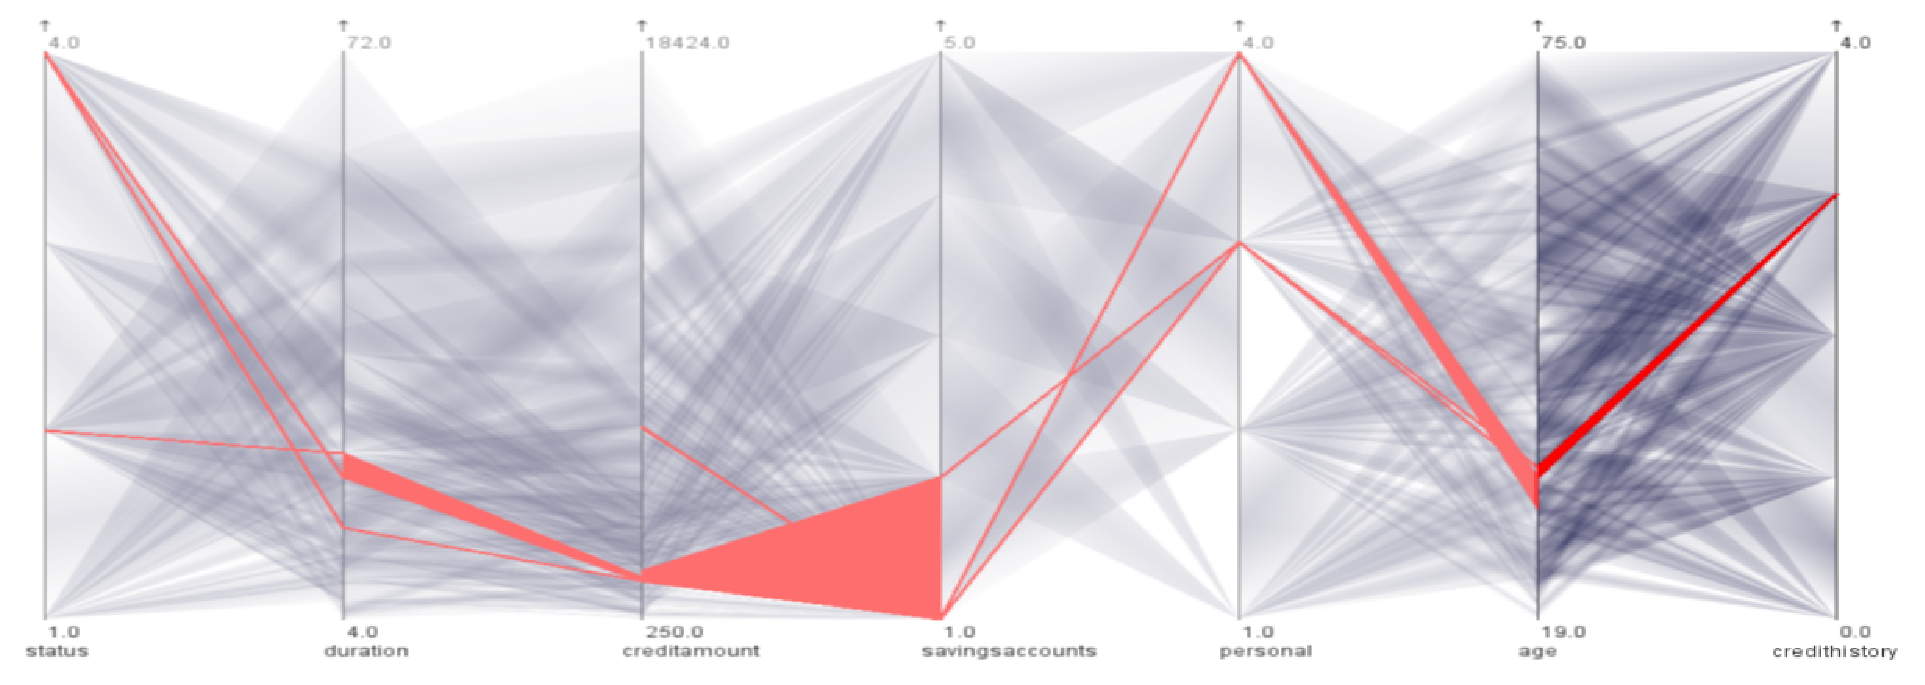
\includegraphics[width=1.0\linewidth]{images/PC_Data_Privacy.eps}
\caption{\label{fig:PC_Data_Privacy}通过聚类保护数据隐私,其中高亮的部分由于存在不确定性而难以理解。本图来源于Dasgupta等人的论文~\citep{dasgupta2011adaptive}~。
}
\end{figure}

\subsubsection{绘制效率}

当数据量较大时,直接绘制的效率较低,容易导致交互过程的延迟。Rosenbaum等人~\citep{rosenbaum2012progressive}提出建立数据的精度层级(Data Hierarchy),在绘制完成前通过低精度小规模的数据来提供概要信息,以平衡信息量与绘制效率(如图~\ref{fig:PC_Data_Splatting})。

\begin{figure}[!htb]
\centering
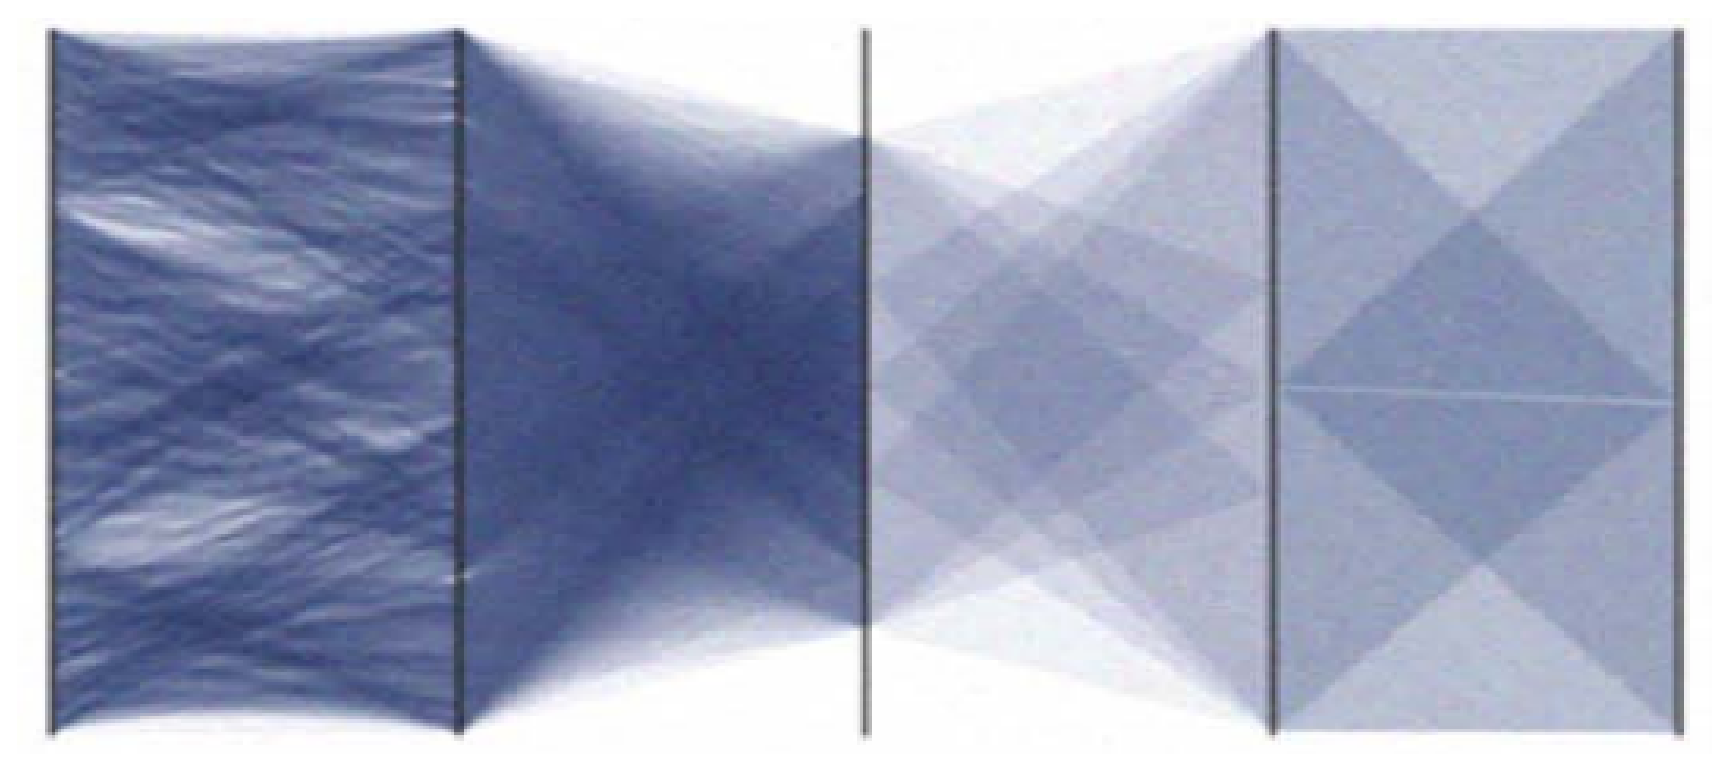
\includegraphics[width=0.8\linewidth]{images/PC_Data_Splatting.eps}
\caption{\label{fig:PC_Data_Splatting}递进式平行坐标,用户可以根据需要指定数据的精度。本图源自Rosenbaum等人的论文~\citep{rosenbaum2012progressive}~。
}
\end{figure}

但在视图精度不断提高的过程中,每个层级的数据都需要重新获取与绘制, 使得自顶向下绘制的总体效率比直接绘制更低。Heinrich等人~\citep{heinrich2011progressive}提出自底向上地渲染连续型平行坐标的方式。他们对数据域进行再采样,通过不断增加的样本来重现、而非直接计算密度分布,从而用户在采样的早期就可看出数据分布的特点。

\subsection{视图}
\label{subsection:designImpro}

如\ref{subsection:designBasics}节所述,对视图设计的研究主要关注三个问题,分别是数据重合、视觉混杂以及坐标轴的排序。

\subsubsection{数据重合}

数据重合的主要问题是无法在视觉上区分多个数据。Graham等人~\citep{graham2003using}提出用曲线代替折线,从而在重合点处,用户可以通过曲率的连续性来跟踪数据(图\ref{fig:PC_Design_Curve1});将重合点展开则可以进一步减轻这一问题(图\ref{fig:PC_Design_Curve2})。

\begin{figure}[!htb]
\centering
\subfigure[]{\label{fig:PC_Design_Curve1}
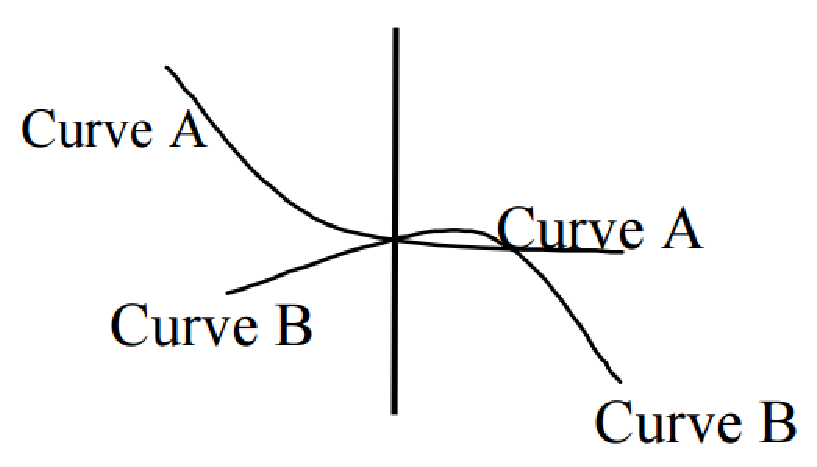
\includegraphics[width=0.58\linewidth]{images/PC_Design_Curve.eps}}
\subfigure[]{\label{fig:PC_Design_Curve2}
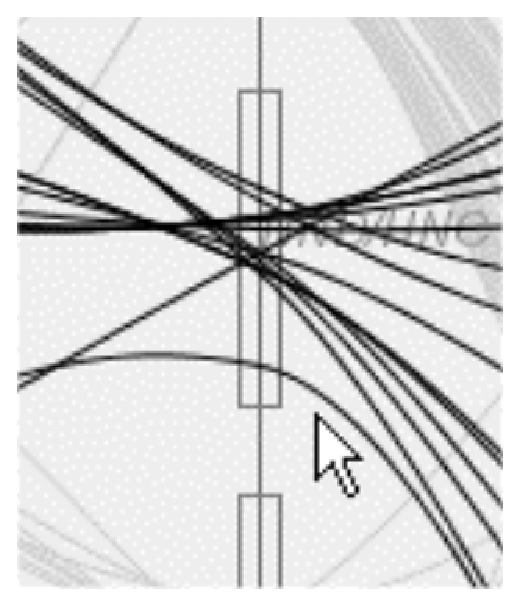
\includegraphics[width=0.28\linewidth]{images/PC_Design_Curve1.eps}}
\caption{通过曲率连续性区分不同数据。本图源自Graham等人的论文~\citep{graham2003using}~。}
\end{figure}

\begin{figure}[!htb]
\centering
\subfigure[]{
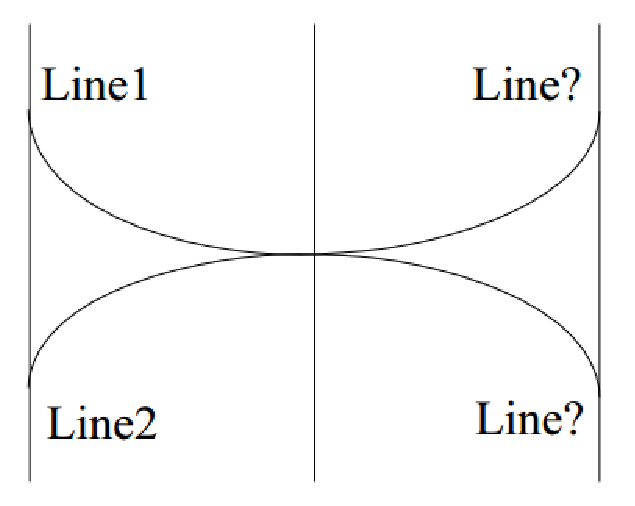
\includegraphics[width=0.37\linewidth]{images/PC_Design_Curve3.eps}}
\subfigure[]{
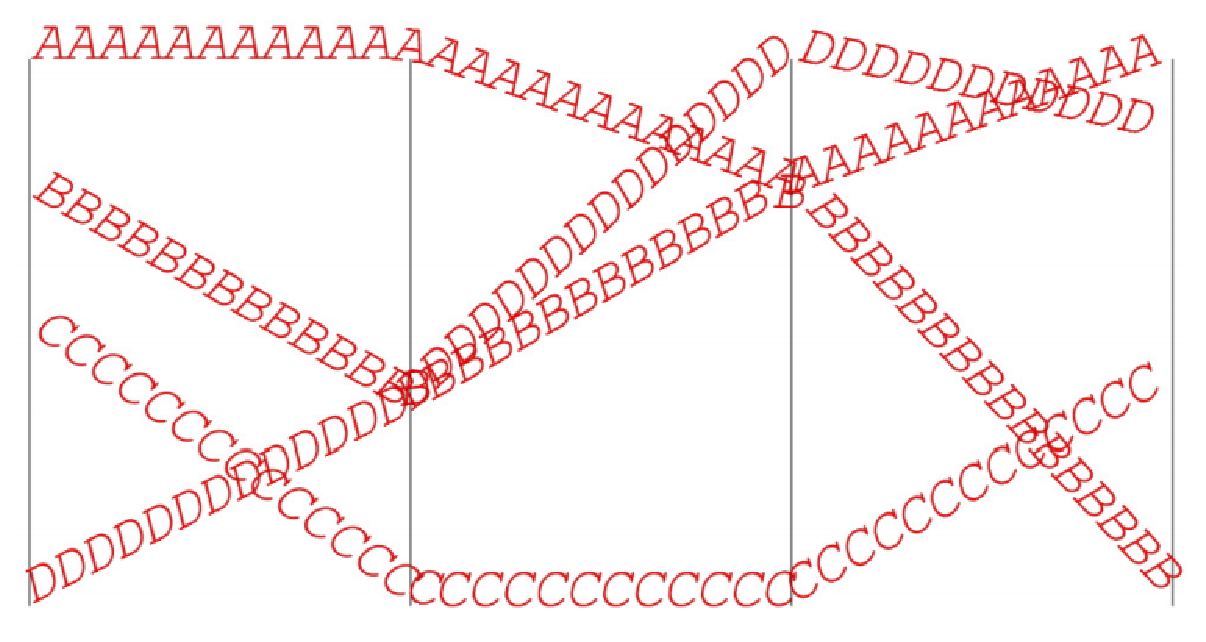
\includegraphics[width=0.57\linewidth]{images/PC_Design_Curve4.eps}}
\caption{\label{fig:PC_Design_Label}平行坐标中的数据标签。本图源自Zhou等人的论文~\citep{zhou2014parallel}~。}
\end{figure}

而Zhou等人~\citep{zhou2014parallel}指出,在重合点处相切的曲线依然无法区分。他们提出用数据标签代替线段(如图\ref{fig:PC_Design_Label}),从而不论是直线或曲线,用户在放大视图时,总能通过标签的不同来区分数据。但标签相比于线段更容易相互遮挡、影响可读性,使得该方法不适合数据量大的情形。

\subsubsection{视觉混杂}

视觉混杂问题是平行坐标研究的重点之一。要在有限的空间里表现大量的图元,主要有五种方法:刻画密度、视觉概要、聚类表达、数据采样、以及扩充
显示空间。其中中间三种都致力于减少图元数目,有异曲同工之处。

密度分布可以是图元或数据的密度,并借由不透明度或色调来表达。表现图元密度的最简单方法,是调节折线的不透明度,从而折线越密集的区域可见性越高(如图~\ref{fig:PC_Data_Time3}(b))。也可以基于屏幕像素来统计折线堆叠的情况,再利用不透明度~\citep{artero2004uncovering}~\citep{johansson2007depth}或色调~\citep{mcdonnell2008illustrative}来呈现(如图~\ref{fig:PC_Design_Density1})。

\begin{figure}[!htb]
\centering
\subfigure[]{
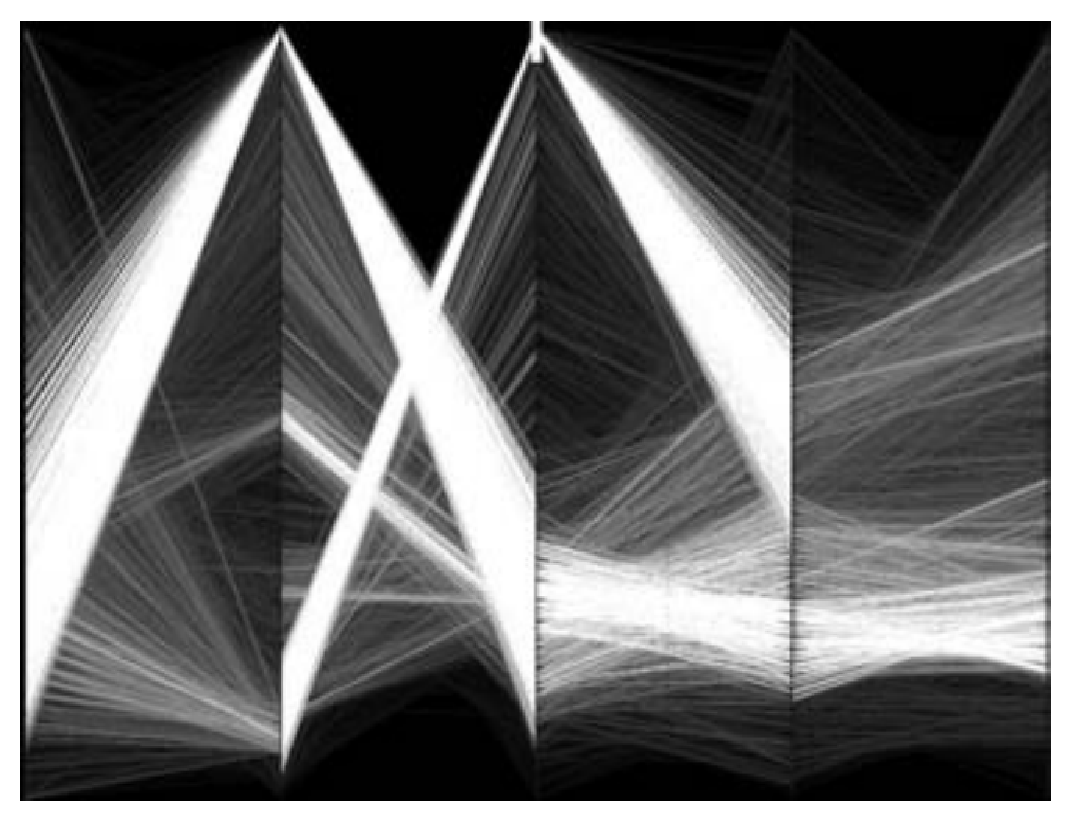
\includegraphics[width=0.4\linewidth]{images/PC_Design_Density1.eps}}
\subfigure[]{
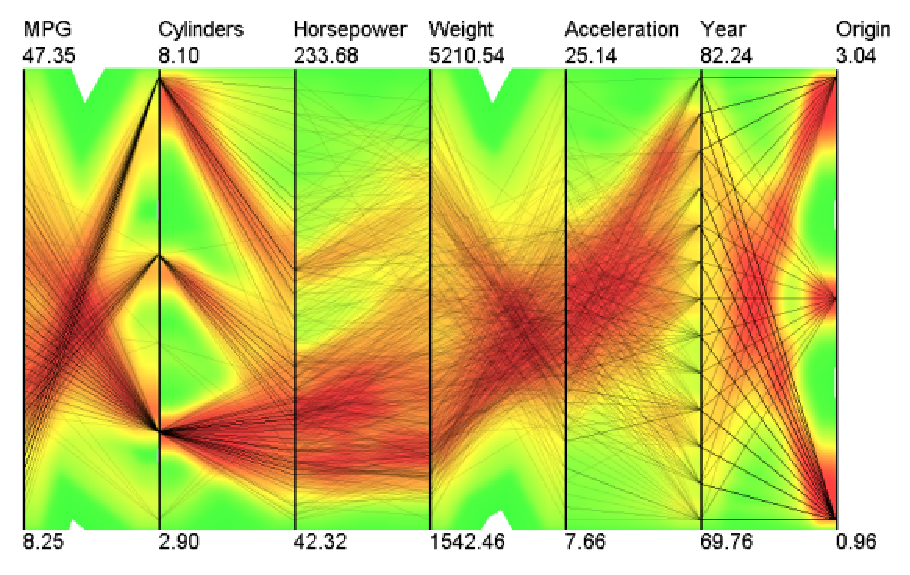
\includegraphics[width=0.55\linewidth]{images/PC_Design_Density2.eps}}
\caption{\label{fig:PC_Design_Density1}利用不透明度或色调表现折线密度}
\end{figure}

然而在平行坐标里,对视图作密度估计并不反映数据域本身的密度。Zhou等人~\citep{zhou2009splatting}提出用抛雪球算法来检测数据聚类,并逐步显现其中的密度分布(如图~\ref{fig:PC_Design_Density2})。

\begin{figure}[!htb]
\centering
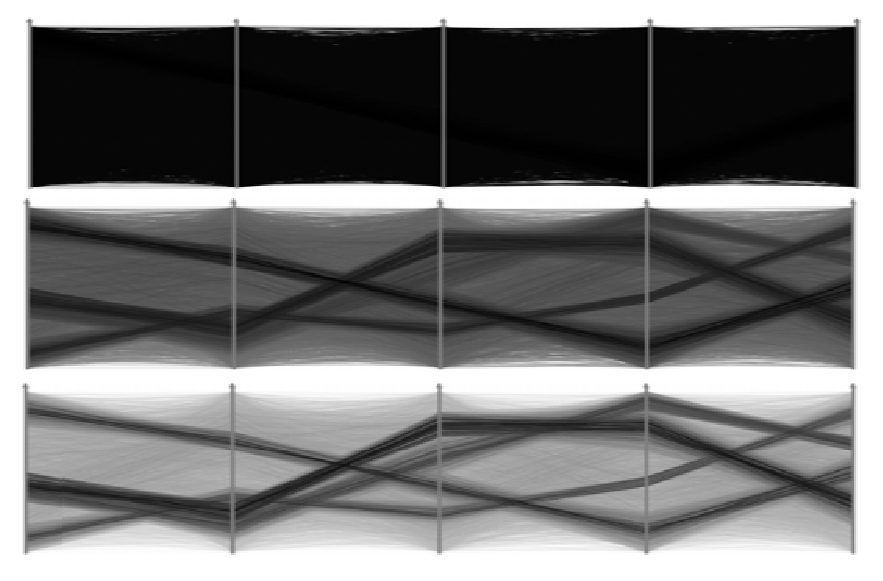
\includegraphics[width=0.8\linewidth]{images/PC_Design_Density3.eps}
\caption{\label{fig:PC_Design_Density2}利用抛雪球算法逐步凸显数据密度。本图修改自Zhou等人的论文~\citep{zhou2009splatting}~。
}
\end{figure}

进一步地,连续型平行坐标的相关研究~\citep{heinrich2009continuous}~\citep{lehmann2011features}~\citep{feng2010matching}~\citep{heinrich2011progressive}直接对数据域作密度估计,并揭示了相应的绘制方式(见图~\ref{fig:PC_Data_Continuous2}、图~\ref{fig:PC_Data_Uncertainty})。如此一来,既无需费时绘制所有数据,避免了混杂问题,又能较好地保留数据分布的信息。然而在上述方法中,低密度区域的信息会因为较低的可见性而被忽略。Johansson等人~\citep{johansson2005revealing}利用传递函数(Transfer Function)来调节密度与可见性的关系,从而用户可以根据分析需求来强调不同密度的区域。

\subsubsection{坐标轴排序}

\subsection{感知}
\label{subsection:perceptionImpro}

\subsection{交互}
\label{subsection:interactionImpro}

\section{平行坐标的应用}
\label{section:applications}

\section{探讨与展望}
\label{section:challenges}

\section{结论}
\label{section:conclusion}

\bibliographystyle{abbrvnat}
%\setcitestyle{aysep={,},yysep={;}}
\bibliography{parallelcoordinates}
	
\end{CJK*}
\end{document}

